\chapter{Collecting Specimens} % see BIO LASM


\section{Methods of Collecting and Displaying}

\begin{multicols}{2}

\subsection{Pitfall Traps}

\begin{center}
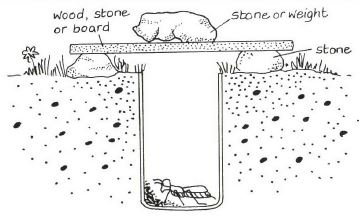
\includegraphics[width=0.45\textwidth]{./img/vso/pitfall.jpg}
\end{center}

\begin{itemize}
\item Make a few holes in the bottom
of a tin to let water escape.
\item Bury the tin up to its rim in the
soil.
\item Cover the tin to keep out rain.
\item Try out different types of food
as bait.
\item Check the trap regularly and
remove it when finished with!
\end{itemize}


\subsection{Worm Jar}

\begin{center}
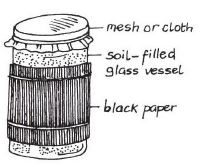
\includegraphics[width=0.4\textwidth]{./img/vso/worm-jar.jpg}
\end{center}

\begin{itemize}
\item Fill a plastic or glass vessel with soil and add the worms.
\item Wrap black or dark paper
around the jar to keep light
away from the burrowing
worms.
\item Remove the paper to reveal the
burrows.
\item Make sure the soil is kept moist
and never dries out.
\end{itemize}


\subsection{Collecting Nets}

\begin{center}
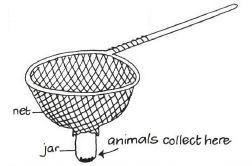
\includegraphics[width=0.45\textwidth]{./img/vso/nets.jpg}
\end{center}

\begin{itemize}
\item Collecting nets can be made easily from sticks, some wire and
mosquito netting.
\item For collecting small water creatures use a fine net with a small jar
attached to the blind end as shown.
\item River nets can be used to catch small animals disturbed from stones
and mud by a stick.
\end{itemize}


\subsection{Soil Life}

\begin{center}
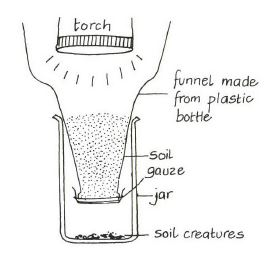
\includegraphics[width=0.35\textwidth]{./img/vso/soil-life.jpg}
\end{center}

\begin{itemize}
\item Collect a sample of soil and
place it in a funnel with a piece
of gauze across its neck.
\item Shine a bright light down onto
the soil.
\item Soil organisms usually prefer
dark, damp and cool conditions
so the heat and light drives
them downwards until they
drop into the collecting jar.
\item Return organisms to the soil
after examination, as many may
dehydrate and die.
\end{itemize}


\subsection{Flying Insect Cage}

\begin{center}
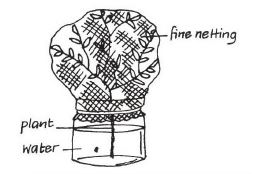
\includegraphics[width=0.45\textwidth]{./img/vso/fly-cage.jpg}
\end{center}

\begin{itemize}
\item Insects can be kept in many
types of cage.
\item Mosquitoes and other insects
benefit from having water,
vegetation and room to fly. The
cage shown provides all these.
\end{itemize}


\subsection{Reptile Cage}

\begin{center}
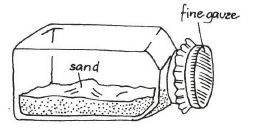
\includegraphics[width=0.45\textwidth]{./img/vso/reptile-cage.jpg}
\end{center}

\begin{itemize}
\item What would you need to add to
this jar to make it suitable for
keeping and observing lizards
or other reptiles?
\end{itemize}


\subsection{Aquarium Box}

\begin{center}
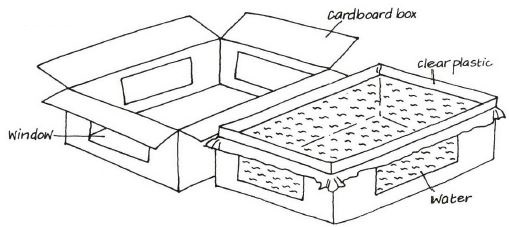
\includegraphics[width=0.49\textwidth]{./img/vso/aquarium.jpg}
\end{center}

\begin{itemize}
\item Cut viewing windows in the
sides of a box.
\item Line the box with a large sheet
of transparent plastic and fill it
with water.
\item Attach the plastic firmly,
making sure it does not slip
down from around the rim of
the box.
\end{itemize}


\subsection{Caring for Animals}

\begin{center}
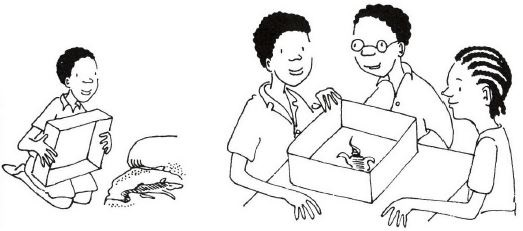
\includegraphics[width=0.49\textwidth]{./img/vso/caring-animals.jpg}
\end{center}

\begin{itemize}
\item Always treat animals with care.
\item Some animals are dangerous,
some scare easily.
\item After study return animals to
the place you found them.
\end{itemize}

\end{multicols}







\pagebreak

\setcounter{secnumdepth}{3}
%\setlength{\parskip}{0.1cm plus0cm minus0cm}
%\onehalfspacing


\section{O-Level Biology Specimens}

When teaching Classification, we will need a variety of organisms that may not always be available. Below is information about each Kingdom, Phylum, and Class on the O-level syllabus  and how to collect, preserve, kill, and dissect examples in each.

\subsection{Kingdom Fungi}
The following are features of Kingdom Fungi:
\begin{enumerate}
\item{They have no roots, stems, or leaves.}
\item{They lack chlorophyll, are non-photosynthetic and have to get their own food by feeding on dead plants or animals. (Notice the lack of green colour, because of lack of chlorophyll)}.
\item{Most fungi have cell walls made of chitin, which is a polysaccharide.}
\item{Their body is made of a network of small, tube-like filaments called hyphae.}
\item{Fungi store carbohydrates as glycogen.}
\item{Fungi reproduce asexually by small structures called spores.} 
\end{enumerate}

There are 3 major phyla in Kingdom Fungi. These are Phylum Basidiomycota, Zygomycota, and Ascomycota.

\begin{multicols}{2}

\subsubsection{Phlyum Basidiomycota}

\textbf{Mushrooms and Toadstools (Uyoga)}\\
Basidiomycota is the most common division of the Fungi Kingdom. Mushrooms and toadstools are in this division. The part of the mushroom that grows above the ground is the reproductive body and is divided into a stem, cap, and gills. Spores are released from the gills and are dispersed by wind.

\paragraph{Collection}
Mushrooms should be collected during the rainy season. Mushrooms can be found on dead and decaying materials like logs in the forest. Mushrooms may also be purchased in supermarkets.

\paragraph{Preservation} 
Dry mushrooms in sunlight or preserve them in alcohol (a clear methylated spirit that is 70 \% alcohol and 30 \% water).

\paragraph{Dissection}
For the dissection of a mushroom, remove the cup of the mushroom and observe the gills. Cut the stem vertically with a razor blade and observe the inside.

\subsubsection{Phylum Zygomycota}

\textbf{Bread Mould and Mucor (Ukungu wa mkate, ukungu wa muhogo)}\\
Zygomycota grows on rotting material and looks like small white thread. An example of Zygomycota is bread mould or mucor.

\paragraph{Collection}

Bread mould may be cultured by exposing some slices of bread to moisture. If you live in a dry area, add a few drops of water to the bread and close in a clear bag.
For mucor culture from fruits like tomatoes, keep in warm and moist conditions. In dry areas, enclose in clear bags. 

\subsubsection{Phylum Ascomycota}

\textbf{Yeast (Hamira)}\\
Ascomycota are single-celled organisms called yeast that grow on the surface of rotting fruit and reproduce by budding. Yeast is used to bake bread and create alcohol.

\paragraph{Collection}
Yeast can be purchased at any shop.

\paragraph{Preservation} 
Keep yeast in an air-tight container.

\end{multicols}


\subsection{Kingdom Plantae}
Organisms in Kingdom Plantae are eukaryotic. Kingdom Plantae is very large and contains many plants.
Although organisms in this group look very different, they all get their nutrition from a process called photosynthesis. Photosynthesis is a way to manufacture food from simple materials with the help of the sun.
 The following are features of Kingdom Plantae:
\begin{enumerate}
\item{In all plants, the cell walls are made up of cellulose.}
\item{They demonstrate autotrophic nutrition -- they manufacture their own food through photosynthesis.}
\item{They have chlorophyll.}
\item{They are multicellular and the plant body is separated into tissues, organs, and systems.}
\end{enumerate}

There are 4 major divisions in Kingdom plantae. These are Division Bryophyta, Filiciniophyta, Coniferophyta, and Angiospermophyta.

\begin{multicols}{2}

\subsubsection{Division Bryophyta}
\textbf{Mosses and Liverworts}\\
Bryophyta are mosses and liverworts. They live on the land, but can only grow in wet places because they have no way to carry water. They also need water to reproduce.\\
These are the features of Division Bryophyta:
\begin{enumerate}
\item{They have no true roots, stems, or leaves.}
\item{They have no vascular tissue.}
\item{They reproduce by using spores.}
\end{enumerate}

\paragraph{Collection}
In dry places, moss should be collected during the rainy season. Moss and liverwort can be found on rocks or trees in moist climates or in rocky riverbanks. 

\paragraph{Preservation} 
Once moss or liverwort has been collected, it can be kept for several days on a rock placed in a container with water.

\subsubsection{Division Filicinophyta}
\textbf{Ferns}\\
Division Filicinophyta are ferns. Ferns grow in moist, shady environments like ground beds of forests. \\
The following are the features of Division Filicinophyta:
\begin{enumerate}
\item{They have true roots, stems, and leaves.}
\item{They have vascular tissue (xylem and phloem).}
\item{The leaves make sori which will later produce spores so the fern can reproduce.}
\item{The leaves are called fronds.}
\item{They grow in damp and shady places.}
\end{enumerate}

\paragraph{Collection}
Ferns can be found in shady and humid environments, usually in forests. 

\paragraph{Preservation} 
Ferns can be dried inside a book for future use. Place a fern between two pieces of paper and then place them into a book. Add more weight on top of the book and wait a few weeks. These specimens will be very delicate but will last a long time.

\subsubsection{Division Coniferophyta}
\textbf{Pine Trees (Mivinje)}\\
 Coniferophyta is a division of Kingdom Plantae. Coniferophyta are cone bearing plants with needle-shaped leaves. The male cones are smaller and produce a yellow powder called pollen. The female cones are larger and have small seed-like structures called ovules.\\
The following are the features of Division Coniferophyta:
\begin{enumerate}
\item{They are mostly shrubs and trees with needle shaped leaves.}
\item{Their reproductive structures are cones.}
\item{The ovule are not enclosed inside an ovary wall.}
\item{The majority are evergreens, which means they keep their leaves all year round.}
\end{enumerate}

\paragraph{Collection}
Coniferophyta can be found in cooler, higher climates like Mbeya, Iringa, and Lushoto. Choose a branch that includes both needle shaped leaves and a cone.

\paragraph{Preservation} 
Coniferophyta can be dried in the sun and stored in a dry place for future use.

\subsubsection{Division Angiospermophyta}
\textbf{Flowering Plants (mimea itoayo maua)}\\ 
Division Angiospermophyta consists of all flowering plants. \\
The following are the features of Division Angiospermophyta:
\begin{enumerate}
\item{Their reproductive structures are flowers.} 
\item{Ovules are enclosed in an ovary and seeds are enclosed in a fruit.}
\end{enumerate}

Division Angiospermophyta can be divided into two classes; Monocotyledons and Diocotyledons.

\setcounter{secnumdepth}{4}

\paragraph{\textbf{Monocotyledons}}
Monocotyledon seeds have only one cotyledon. Monocots have a fibrous root system, leaves with parallel venation, three part floral systems, and vascular bundles which are scattered. Examples of monocotyledons are maize and grasses.

\paragraph{\textbf{Dicotyledons}}
Dicotyledons seeds have two cotyledons. They also have a tap root system, leaves with net-like veins, floral parts in four or fives, and vascular bundles which form a ring in the stem. Examples of dicotyledons are mangoes, cashews, beans, and okra.

\subparagraph{Collection}
Angiosperms are easily found in your surrounding environment. Monocotyledons are organisms like maize plants and grasses. Dicotyledons are organisms like mango trees, cashew nut trees, and okra.

\subparagraph{Preservation} 
Flowers and leaves can be dried in a book. Place the flower or leaf between two sheets of paper and then press these in the centre of a book. Place the book in a safe place and add more books on top. Leave for a few weeks and then remove.

\subparagraph{Dissection}
Hibiscus flowers can be easily dissected using a razor blade to identify the reproductive parts.

\end{multicols}

\setcounter{secnumdepth}{3}

\subsection{Kingdom Animalia}
Organisms in Kingdom Animalia are eukaryotic. There are many organisms and phyla in Kingdom Animalia. However, for practical purposes, students will only study Phylum Platyhelminthes, Annelida, Nematoda, Arthropda, and Chordata.\\
The following are the features of Kingdom Animalia:
\begin{enumerate}
\item{Animals are multicellular.}
\item{Animals are differentiated into tissues.}
\item{Animals are heterotrophic feeders.}
\item{Animals are capable of locomotion.}
\item{Animals have a nervous system (with the exception of sponges.)}
\end{enumerate}


\begin{multicols}{2}

\subsubsection{Phylum Platyhelminthes}
\textbf{Flatworms}\\ 
Phylum Platyhelminthes defining characteristic is that their bodies are dorso-ventrally flattened and most are parasitic and feed off other organisms.\\
This phylum is divided into three classes: Trematoda (Flukes), Cestoda (Tapeworms), and Turbellaria.
\begin{enumerate}
\item{Class Trematoda or flukes (minyoo bapa) are parasitic. They are flat and use suckers to feed.}
\item{Class Cestoda or tapeworms (minyoo yenye pingili) are flat, tape-like and have segmented or divided bodies. They are parasitic and use suckers and hooks to feed. Tapeworms live in the human intestines and affect humans by absorbing partly digested food. They can cause disease as well as malnutrition.}
\item{Class Turbellaria are flat and have cilia which help them move.}
\end{enumerate}

\paragraph{Collection}
 Flukes can be collected when a cow, pig, or sheep is slaughtered by examining the liver or intestines. There are some species of flatworm that can be found in shallow tide pools along the beach. 

\paragraph{Preservation} 
Organisms in Phylum Platyhelminthes can be kept in labelled air-tight containers with formaldehyde solution.

\paragraph{Killing}
Place the Platyhelminthes into a formaldehyde solution.

\paragraph{Dissection}
You can observe the unbranched gut of a Plathelminthes by making a lateral cut along the body and observing the internal structure of the organism.

\subsubsection{Phylum Nematoda or Ascehelminthyes}
\textbf{Roundworms}\\
Phylum Nematoda, also known as Aschelminthyes, includes round parasitic worms that cause infections in humans.\\
The following are the features of the Phylum Nematoda 
\begin{enumerate}
\item{They have unsegmented, cylindrical bodies with pointed ends.}
\item{Their body is covered in a cuticle of protein.}
\item{They have an unbranched gut from mouth to anus.}
\end{enumerate}

\paragraph{Collection}
Roundworms can be found in the stomach of fish, in soil or stagnant water, or in the intestines of locally raised chicken.

\paragraph{Preservation} 
Organisms in Phylum Nematoda can be kept in labelled air-tight containers with formaldehyde solution.

\paragraph{Killing}
Place the Nematoda into a formaldehyde solution.

\paragraph{Dissection}
You can observe the unbranched gut of a Nematoda by making a lateral cut along the body and observing the internal structure of the organism.

\subsubsection{Phylum Annelida}
\textbf{Earthworms (Chambo) and Leeches (Ruba)}\\ 
Phylum Annelida are eukaryotic organisms. Earthworms have a mouth at their anterior end and anus at the posterior end with a bulge called a clitellum in the middle that holds eggs. The earthworm uses bristles (small hair like structures) to burrow through the dirt. \\
The following are the features of the Phylum Annelida:
\begin{enumerate}
\item{They are segmented. They have separate internal organs and body walls.}
\item{They have a thin, moist, non-chitinous cuticle.}
\item{Their body has external bristles.}
\end{enumerate}

\paragraph{Collection}
Earthworms can be found after a rain by digging under rocks or in other damp places. Leeches can be found in a river.

\paragraph{Preservation} 
You can keep earthworms in a container with fresh soil to preserve live specimens. If killed, these organisms can be preserved in ethanol alcohol for a few months. 

\paragraph{Killing}
Place the Annelida into a closed bottle in which is suspended a ball of cloth or mosquito net soaked in methylated spirits. Avoid direct contact with the spirit

\paragraph{Dissection}
You can observe the internal structures of an earthworm by making a lateral cut along the body.

\begin{center}
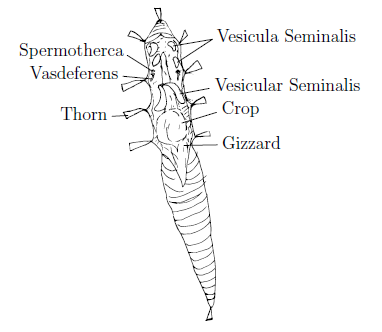
\includegraphics[width=0.45\textwidth]{./img/earthworm.png}
\end{center}

%\begin{figure}[h]
%\centering
%%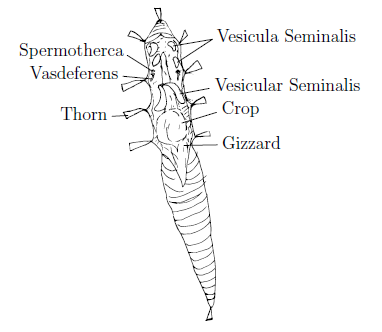
\includegraphics[width=0.45\textwidth]{./img/earthworm.png}
%\def\svgwidth{8cm}
%\input{./img/worm-dissection.pdf_tex}
%\caption{Dissection of Earthworm}
%\label{fig:worm-dissection}
%\end{figure}

\subsubsection{Phylum Arthropoda}
Organisms in this phylum have jointed appendages and an exoskeleton made of chitin. There are 5 classes in this phylum: Insecta, Crustecea, Arachnida, Diplopoda, and Chilopoda.

\setcounter{secnumdepth}{4}

\paragraph{Class Insecta}
\textbf{Beetles, Houseflies (Nzi), Grasshoppers (Panzi), Ants (Sisimizi), and Termites (Mchwa)}\\
The following are the features of Class Insect:
\begin{enumerate}
\item{Insects have a head, thorax, and abdomen.}
\item{They have one pair of antennae.}
\item{They have three pairs of jointed legs.}
\item{Most adult insects have wings.}
\end{enumerate}

\subparagraph{Collection}
Many insects can be caught in a field using a sweep net. 

\subparagraph{Preservation} 
Live insects can be kept in a clear bottle and fed grass clippings. Dead insects can be preserved for a few months by placing them in methylated spirits.

\subparagraph{Killing}
Seal in an airtight container until the insect suffocates.

\subparagraph{Dissection}
First remove wings, antenae, and legs of the insect. Then cut down the sides of the insect to open the body cavity and observe the digestion and reproductive systems.
	
\paragraph{Class Crustacea}
\textbf{Crabs (Kaa), Prawns (Kamba), and Lobsters (Kamba Kochi)}\\
The following are the features of Class Crustacea:
\begin{enumerate}
\item{Crustacea have bi-forked appendages.}
\item{They have 2 pairs of antennae.}
\end{enumerate}

\begin{center}
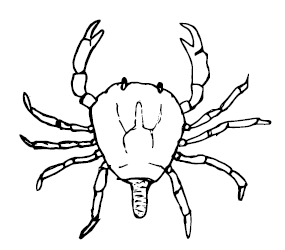
\includegraphics[width=0.4\textwidth]{./img/crab.png}
\end{center}

%\begin{figure}[h]
%\begin{center}
%\def\svgwidth{6cm}
%\input{./img/crab.pdf_tex}
%\caption{Crabs are an example of Class Crustacea}
%\label{fig:crab}
%\end{center}
%\end{figure}

\subparagraph{Collection}
Fresh water crabs, prawns, and shrimp can be found in most rivers, lakes, dams and swamps. Otherwise, they can be purchased in many markets.


\subparagraph{Preservation} 
Crustacea can be preserved in methylated spirits. Crustacea can also be dried for preservation purposes.

\subparagraph{Killing}
Crustesea can be killed by being left in an airtight container or boiled in water.

\subparagraph{Dissection}
For crabs, turn it so that its abdomen is facing up. Wedge a knife under the triangular abdomen and twist, so that the abdomen opens. Examine the internal organs.
		
\paragraph{Class Arachnida}
\textbf{Spiders (Buibui) and Scorpions (Nge)}\\
The following are the features of Class Arachnida:
\begin{enumerate}
\item{Arachnids have four pairs of jointed legs.}
\item{Arachnids have a cephalothorax (head and thorax) and abdomen.}
\end{enumerate}

\begin{center}
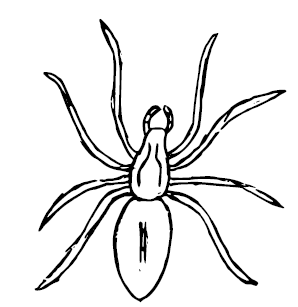
\includegraphics[width=0.35\textwidth]{./img/spider.png}
\end{center}

%\begin{figure}[h]
%\begin{center}
%\def\svgwidth{6cm}
%\input{./img/spider.pdf_tex}
%\caption{Spiders are an example of Class Arachnida.}
%\label{fig:fish}
%\end{center}
%\end{figure}

\subparagraph{Collection}
Spiders can be found in almost any environment. Scorpions can be found in dark, dry and cool areas, usually at night.

\subparagraph{Preservation} 
Arachnida can be dried or preserved in methylated spirits.

\subparagraph{Killing}
To kill Archnida, place them in an airtight container for a few days or use insecticide.
		
\paragraph{Class Chilopoda}
\textbf{Centipedes (Tandu)}\\
The following are the features of Class Chilopoda:
\begin{enumerate}
\item{Chilopoda have long bodies consisting of many segments.}
\item{Each segment contains a pair of legs.}
\end{enumerate}

\begin{center}
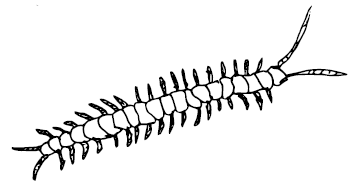
\includegraphics[width=0.4\textwidth]{./img/centipede.png}
\end{center}

%\begin{figure}[h]
%\begin{center}
%\def\svgwidth{8cm}
%\input{./img/centipede.pdf_tex}
%\caption{A centipede}
%\label{fig:centipede}
%\end{center}
%\end{figure}

\subparagraph{Collection}
Centipedes can be found under rocks, in tree bark, and in leaf litter.

\subparagraph{Preservation} 
Chilopoda can be dried or preserved in methylated spirits.

\subparagraph{Killing}
To kill Chilopoda, place them in an airtight container for a few days or use insecticide.

\paragraph{Class Diplopoda}
\textbf{Millipedes (Jongoo)}\\
The following are the features of Class Diplopoda:
\begin{enumerate}
\item{Diplopoda have long bodies consisting of many segments.}
\item{Each segment contains 2 pair of legs.}
\end{enumerate}

\subparagraph{Collection}
Milipedes can be found under rocks, in tree bark, and in leaf litter.

\subparagraph{Preservation} 
Diplopoda can be dried or preserved in methylated spirits.

\subparagraph{Killing}
To kill Diplopoda, place them in an airtight container for a few days or use insecticide.
		
\begin{center}
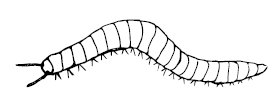
\includegraphics[width=0.4\textwidth]{./img/millipede.png}
\end{center}

%\begin{figure}[h]
%\begin{center}
%\def\svgwidth{6cm}
%\input{./img/millipede.pdf_tex}
%\caption{Class Diplopoda contains organisms like millipedes.}
%\label{fig:Diplopoda}
%\end{center}
%\end{figure}


\subsubsection{Phylum Chordata}
Chordata are eukaryotic organisms that contain a backbone. These organisms have 4 distinct features:
\begin{enumerate}
\item{They have a notochord in the embryonic stage. In most chordates this will be replaced with a vertebral column.}
\item{They have a nerve chord.}
\item{They have gill slits during the embryonic stage.}
\item{They have a tail which is behind the anus.}
\end{enumerate}

In this phylum, there are 6 classes: Chondrichthyes, Osteichthyes, Amphibia, Aves, Reptilia, and Mammalia.

\paragraph{Class Chondrichthyes}
\textbf{Sharks (Papa), Skates (Taa), and Rays}\\
Chondrichthyes are also known as cartilagous fish. Chondrichthyes include sharks, skates, and rays.\\
The features of Class Chondrichthyes are:
\begin{enumerate}
\item{The skeleton is made of cartilage.}
\item{The body is covered with placoid scales.}
\item{The tail fin is asymmetrical.}
\item{The gill slits are visible.}
\item{The mouth and two nostrils are centrally placed.}
\item{They are cold blooded or ectothermic. This means their body temperature changes with the environment.}
\end{enumerate}

\subparagraph{Collection}
Chondrichthyes can be found in most fish markets by the ocean. 

\subparagraph{Preservation} 
Chondrichthyes can be preserved in a formaldehyde solution.

\subparagraph{Killing}
Chondrichthyes can be killed by removing them from water. 

\subparagraph{Dissection}
For sharks, make a lateral cut from the mouth down to the anus. Make another cut from the left pectoral fin to the right. Peel back the layer of skin and examine the internal organs. You can also examine the brain by shaving off thin layers from the top of the head until you reach the brain.

\begin{center}
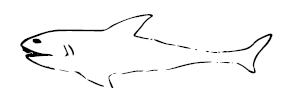
\includegraphics[width=0.4\textwidth]{./img/shark.png}
\end{center}

%\begin{figure}[h]
%\begin{center}
%\def\svgwidth{6cm}
%\input{./img/shark.pdf_tex}
%\caption{A shark}
%\label{fig:shark}
%\end{center}
%\end{figure}

\paragraph{Class Osteichthyes}

\textbf{Tilapia (Sato) and small fish (Dagaa)}\\
Osteichthyes are also known as bony fish. The following are the characteristics of Class Osteichthyes:
\begin{enumerate}
\item{The skeleton is made of bone.}
\item{The body is covered with scales.}
\item{The gills are covered by an operculum.}
\item{The tail fin is symmetrical.}
\item{Most have an air sac or swim bladder.}
\item{They are cold blooded or ectothermic. This means their body changes temperature with the environment.}
\end{enumerate}

\subparagraph{Collection}
 Osteichthyes can be found in both fresh water and the ocean. Fresh killed fish can also be purchased at the fish market.

\subparagraph{Preservation} 
Osteichthyes can be preserved in a formaldhyde solution. Ostechithyes can also be dried and smoked. 
To smoke a fish, make a fire and put fish on a rack over the fire. Smoke the fish until it is dry. This takes from hours to days depending on the size of the fish.

\begin{center}
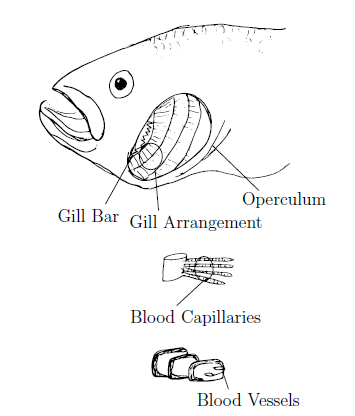
\includegraphics[width=0.4\textwidth]{./img/fish.png}
\end{center}

%\begin{figure}[h]
%\begin{center}
%\def\svgwidth{6.5cm}
%\input{./img/fish-gills.pdf_tex}
%\caption{Have students observe and identify the gills of a fish.}
%\label{fig:fish  gills}
%\end{center}
%\end{figure}

\subparagraph{Killing}
Osteichthyes can be killed by removing them from water. 

\subparagraph{Dissection}
Make a lateral cut from the mouth to the anus of the fish. Open the cut and observe the digestive system. Then, peel back the gill cover, operculum, and observe the structure of the gills.

\paragraph{Class Amphibia}
\textbf{Frog (Chura wa majini), Toad (Chura wa nchi kavu), and Salamander (Boromondo au Tunutunu)}\\The features of this class are:
\begin{enumerate}
\item{They have to spend part of their life in water during the larva stage.}
\item{Their skin is always moist and without scales.}
\item{Their life cycle involves a form called a tadpole.}
\item{They are cold-blooded or ectothermic.}
\end{enumerate}

\subparagraph{Collection}
These organisms can be found near rivers or ponds. Toads can also be collected at night during the rainy season. Use cages or sweep nets to capture amphibians.

\subparagraph{Preservation} 
Make an aquarium or pond for live specimens, providing small insects for food and a source of water. For the preservation of dead specimens inject formaldehyde or leave in the sun for a few days until they are dried.

\subparagraph{Killing}
To kill Amphibians, keep them in an airtight container or prick their head with a nail or pin.

\subparagraph{Dissection}
For frogs, make a lateral cut from the mouth to the anus. Then make two intersecting cuts, one that is under the arms and one that is above the legs. Peel back the layer of skin and observe the internal organs.

\begin{center}
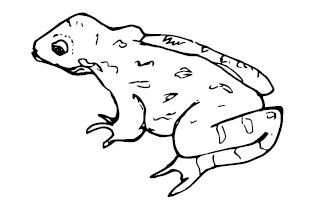
\includegraphics[width=0.4\textwidth]{./img/frog.png}
\end{center}

%\begin{figure}[h]
%\begin{center}
%\def\svgwidth{6cm}
%\input{./img/frog.pdf_tex}
%\caption{Frogs have moist skin and are ectothermic.}
%\label{fig:anae-resp3}
%\end{center}
%\end{figure}

\paragraph{Class Reptilia}
\textbf{Lizards (Mjusi), Crocodiles (Mamba), Snakes (Nyoka), Turtles (Kasa), and Tortoise (Kobe)}\\The following are the features of Class Reptilia:
\begin{enumerate}
\item{They have dry skin with horny scales.}
\item{They are cold blooded or ectothermic.}
\item{They lay their eggs on land and the eggs have a soft shell.}
\end{enumerate}

\subparagraph{Collection}
Reptiles can be found on rocks or in caves, inside cracks in the wall, forests, and in or nearby rivers and lakes.They can be collected by using sweep nets, traps, or fishing nets.

\subparagraph{Preservation} 
Live specimens can be held inside a cage or aquarium. Snakes should be fed small rodents and turtles can be given grass or leaves. For dead specimens, preserve them by placing them in an airtight container with formaldhyde solution.

\begin{center}
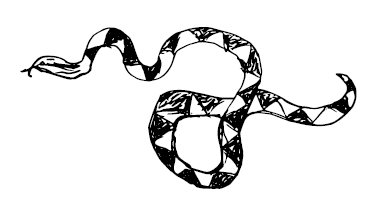
\includegraphics[width=0.4\textwidth]{./img/snake.png}
\end{center}

%\begin{figure}[h]
%\begin{center}
%\def\svgwidth{8cm}
%\input{./img/snake.pdf_tex}
%\caption{Snakes are an example of a reptile.}
%\label{fig:snake}
%\end{center}
%\end{figure}

\subparagraph{Killing}
Reptiles can be killed by placing them in an airtight container, submerging them in bucket of water, or hitting the back of their head with a pin or nail.

\subparagraph{Dissection}
For dissection, follow the same guidelines as amphibian dissection.

\paragraph{Class Aves}

\textbf{Eagle (Tai), Owl (Bundi), Crow (Kunguru), and Chicken (Kuku)}\\ Class Aves contains the organisms commonly known as birds. The following are the features of Class Aves:\\
\begin{enumerate}
\item{Their body is covered with feathers.}
\item{They have wings.}
\item{They have a bill or beak.}
\item{They lay hard-shelled eggs.}
\item{They are warm blooded or homothermic, which means they maintain a constant body temperature.}
\end{enumerate}

\begin{center}
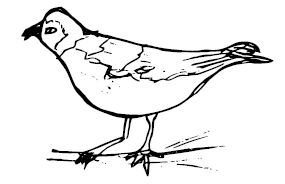
\includegraphics[width=0.4\textwidth]{./img/bird.png}
\end{center}

%\begin{figure}
%\begin{center}
%\def\svgwidth{6cm}
%\input{./img/bird.pdf_tex}
%\caption{Organism in Class Aves}
%\label{fig:bird}
%\end{center}
%\end{figure}

\subparagraph{Collection}
Chicken are kept domestically and can be easily purchased or raised. Wild birds usually live in the forest and can be killed using a sling shot or captured live with the use of a sweep net or fishing net.

\subparagraph{Preservation} 
To preserve dead specimens, place them in an airtight container with formaldehyde solution. You can also keep and dry bones of dead bird for studying.

\subparagraph{Killing}
 To kill birds, break their neck, drown them in water, or use a slingshot.

\subparagraph{Dissection}
Make a lateral cut starting at the lower abdomen up to the sternum. Cut through the rib cage and pin it back to the dissection tray to examine the heart, respriatory system, and digestive system.

\paragraph{Class Mammalia} 
\textbf{Rats (Panya), Cats (Paka), Goats (Mbuzi), Bats (Popo), Whale (Nyangumi), and Humans (Binadamu)}\\
The following are the features of Class Mammalia:
\begin{enumerate}
\item{They have a developed brain.}
\item{They have hair or fur on their body.}
\item{They have mammary glands which in females, produce milk.}
\item{They have teeth.}
\item{They have a diaphragm.}
\item{They are viviparous, which means the fetus develops inside the mother’s body.}
\item{They have sweat glands.}
\item{They are warm blooded or homoeothermic.}
\end{enumerate}

\subparagraph{Collection}
Rats can be captured overnight using a trap. Bats can be collected during the day, when they are sleeping, by using a sweep net.

\begin{center}
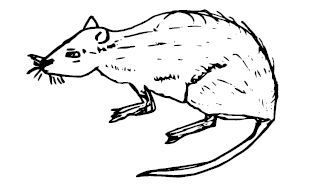
\includegraphics[width=0.4\textwidth]{./img/rat.png}
\end{center}

%\begin{figure}[h]
%\begin{center}
%\def\svgwidth{6cm}
%\input{./img/rat.pdf_tex}
%\caption{Rats are a common example of a mammal and can be used in many dissection activities.}
%\label{fig:rat}
%\end{center}
%\end{figure}

\subparagraph{Preservation} 
Mammals can be preserved in a formaldhyde solution.

\subparagraph{Killing}
Specimens should be killed by drowning. Place the mammal inside a cage or trap and submerge in a bucket of water. Wait at least 10 minutes. After the animal is dead, add one cap full of bleach for every five litres of water in the bucket (e.g. 2 caps of bleach for a 10 litre bucket). Stir the contents of the bucket. Wait 20 minutes. The bleach will kill harmful organisms on the outside of the specimen.

\subparagraph{Dissection}
Make a lateral cut from the mouth to the anus. Then make 2 cuts, one from hand to hand and another from foot to foot so that both cuts cross the first lateral cut. Separate the skin and pin it to the dissection tray to examine the internal organs.

\end{multicols}

\setcounter{secnumdepth}{2}